% ****** Start of file apssamp.tex ******
%
%   This file is part of the APS files in the REVTeX 4.1 distribution.
%   Version 4.1r of REVTeX, August 2010
%
%   Copyright (c) 2009, 2010 The American Physical Society.
%
%   See the REVTeX 4 README file for restrictions and more information.
%
% TeX'ing this file requires that you have AMS-LaTeX 2.0 installed
% as well as the rest of the prerequisites for REVTeX 4.1
%
% See the REVTeX 4 README file
% It also requires running BibTeX. The commands are as follows:
%
%  1)  latex apssamp.tex
%  2)  bibtex apssamp
%  3)  latex apssamp.tex
%  4)  latex apssamp.tex
%
\documentclass[%
 reprint,
%superscriptaddress,
%groupedaddress,
%unsortedaddress,
%runinaddress,
%frontmatterverbose, 
%preprint,
%showpacs,preprintnumbers,
%nofootinbib,
%nobibnotes,
%bibnotes,
 amsmath,amssymb,
 aps,
%pra,
%prb,
%rmp,
%prstab,
%prstper,
%floatfix,
10pt
]{revtex4-1}

\usepackage{color}
\usepackage{graphicx}
\usepackage[caption=false]{subfig}
\usepackage{graphicx}% Include figure files
\usepackage{dcolumn}% Align table columns on decimal point
\usepackage{bm}% bold math
%\usepackage{hyperref}% add hypertext capabilities
%\usepackage[mathlines]{lineno}% Enable numbering of text and display math
%\linenumbers\relax % Commence numbering lines

%\usepackage[showframe,%Uncomment any one of the following lines to test 
%%scale=0.7, marginratio={1:1, 2:3}, ignoreall,% default settings
%%text={7in,10in},centering,
%%margin=1.5in,
%%total={6.5in,8.75in}, top=1.2in, left=0.9in, includefoot,
%%height=10in,a5paper,hmargin={3cm,0.8in},
%]{geometry}

\begin{document}

\preprint{APS/123-QED}

\title{Scattering in atomic and molecular physics \\ AM205 Final Project}% Force line breaks with \\
% \thanks{A footnote to the article title}%

\author{Ben Augenbraun, Andrei Gheorghe, Jessie Zhang}

\date{\today}% It is always \today, today,
             %  but any date may be explicitly specified

\section{\label{sec:level1}Atom + molecule scattering}
\subsection{\label{sec:level1}General approach}

As already discussed, due to the large number of available rovibrational states, doing a full multichannel quantum mechanical study of a reaction even between somehting as simple as a dimer and an atom can be a very complex problem, almost impossible to solve with nowadays capabilities. However, as observed by Croft and Bohn~\cite{bohn2014}, many of the features and observables of a collision between a molecule and a dimer, such as its chaotic behavior or scattering rate, can be computed by using a purely classical approach. This poses a much more tractable problem, both analytically and computationally. 

To perform the classical computation we assume that the interaction is purely determined by a pairwaise-additive Lennard-Jones potential

\begin{equation}
(\mathbf{r_{\mathrm{1}}}, \mathbf{r_{\mathrm{2}}}, \mathbf{r_{\mathrm{3}}}) = \sum_{i \neq j} \frac{C_{\mathrm{12}}}{(\mathbf{r_{\mathrm{i}}}-\mathbf{r_{\mathrm{j}}})^{12}} - \frac{C_{\mathrm{6}}}{(\mathbf{r_{\mathrm{i}}}-\mathbf{r_{\mathrm{j}}})^6},
\label{eq:LJ}
\end{equation}
where $C_{\mathrm{6}}$ is the leading order van der Waals coefficient, and the higher order $C_{\mathrm{12}}$ is chosen in order to obtain the correct atom-atom well depth, as given by $D_{\mathrm{e}} = C_{\mathrm{6}}^2/4D_{\mathrm{e}}$. Other effects such as contributions due to the spin of the atoms are ignored and the values of the van der Waals coefficients used are summarized in Table~\ref{table:coeffs}, where the atom spieces are chosen such as to span a wide range of possible atomic atoms (they are also alkali metals, which are extensively used in ultracold gases experiments). From the potential energy we can readily compute the forces acting on the atoms, $\mathbf{F} = -\mathbf{\nabla}V$, from which we can use Newton's laws to propagate the atoms in time. {\color{red} This last sentence is clunky. Maybe change it?}

\begin{table}
\begin{center}
 \begin{tabular}{|c c c|} 
 \hline
 System & C6 (a.u.) & C12 (a.u.)\\ 
 \hline\hline
$Li + Li$ & 1394 & 1521.8e-6 \\ 
 \hline
 $Cs + Cs$ & 6891 & 1271.2e-6 \\
 \hline
\end{tabular}
\caption{$C_6$ Van der Waals coefficients and well depths $D_e$ for $\mathrm{Li_2}$~\cite{dattani2011} and $\mathrm{Cs_2}$~\cite{xie2009}.}
\label{table:coeffs}
\end{center}
\end {table}

An exaggerated version of the Lennard-Jones potential is given in Fig.~\ref{fig:schematic}, together with the basic setup of the collision's initial conditions. We thus distinguish the orientation of the dimer in the XZ-plane, $\theta_0$, the initial velocity of the incoming atom (in the rest frame of the dimer), as given by the initial temperature $T$, and the impact parameter, $b$, as some of the initial condition variables we can tune in order to analyze the collision. As already mentioned, we can also consider different atomic species, which changes the masses and the interaction strengths.

\begin{figure}[htp]
\subfloat{
  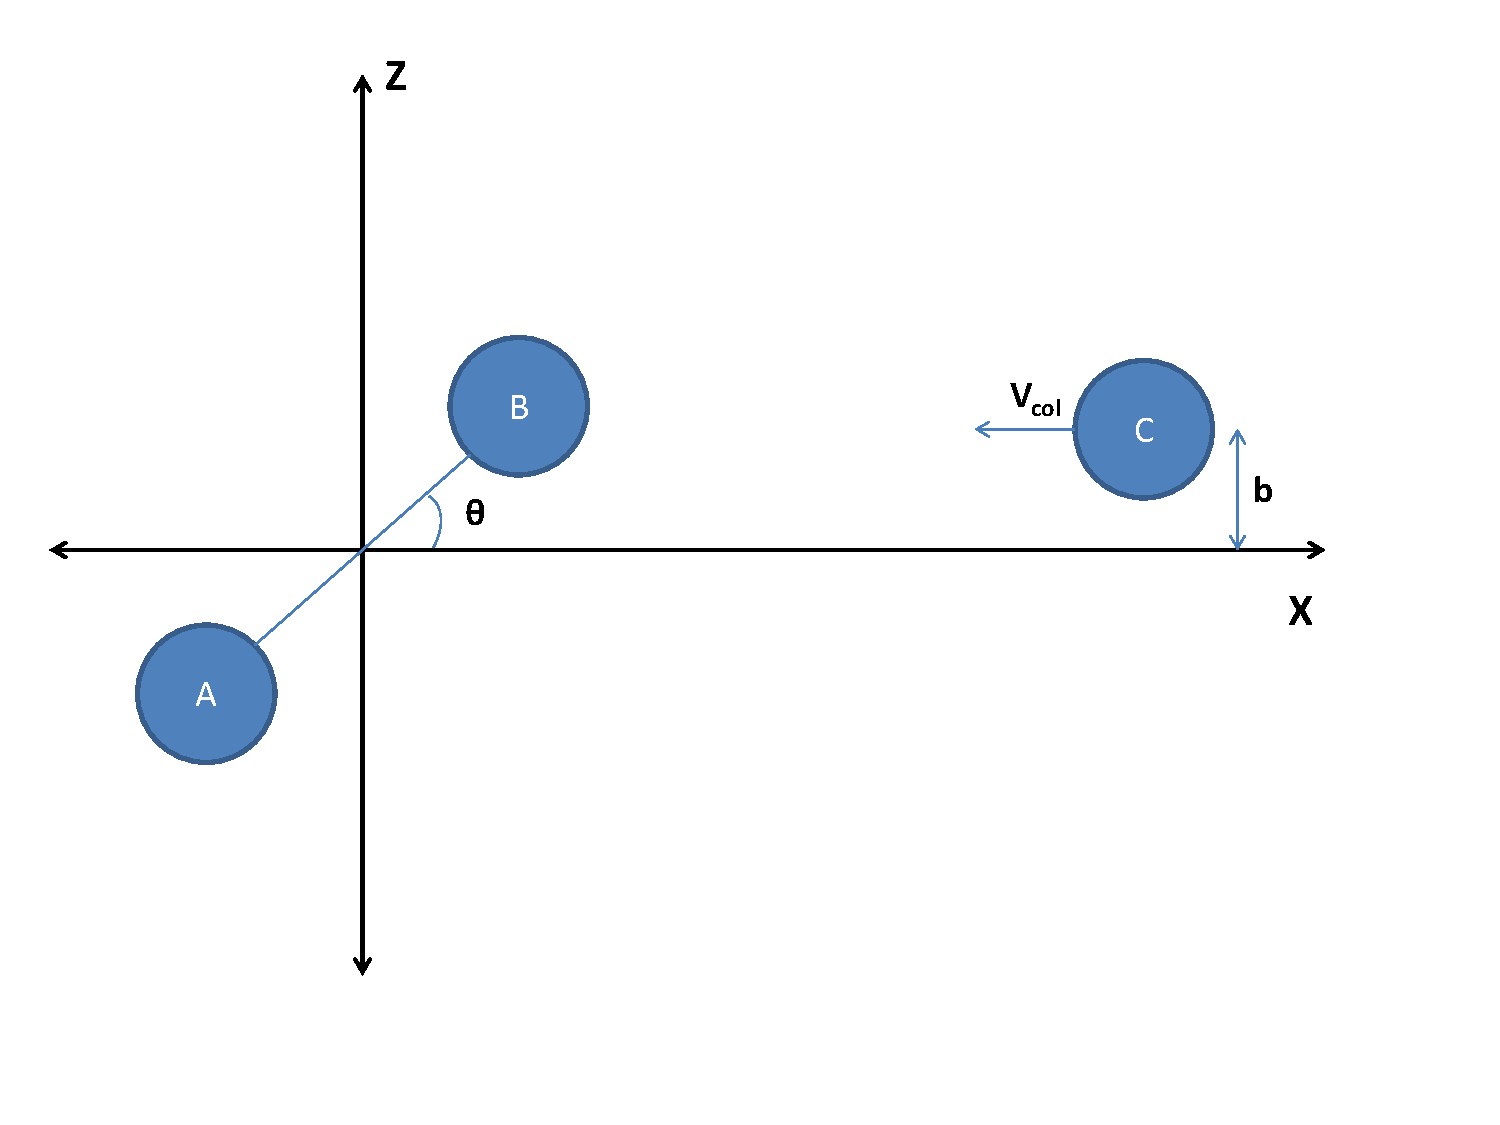
\includegraphics[clip,width=0.85\columnwidth]{schematic.pdf}%
}

\subfloat{
  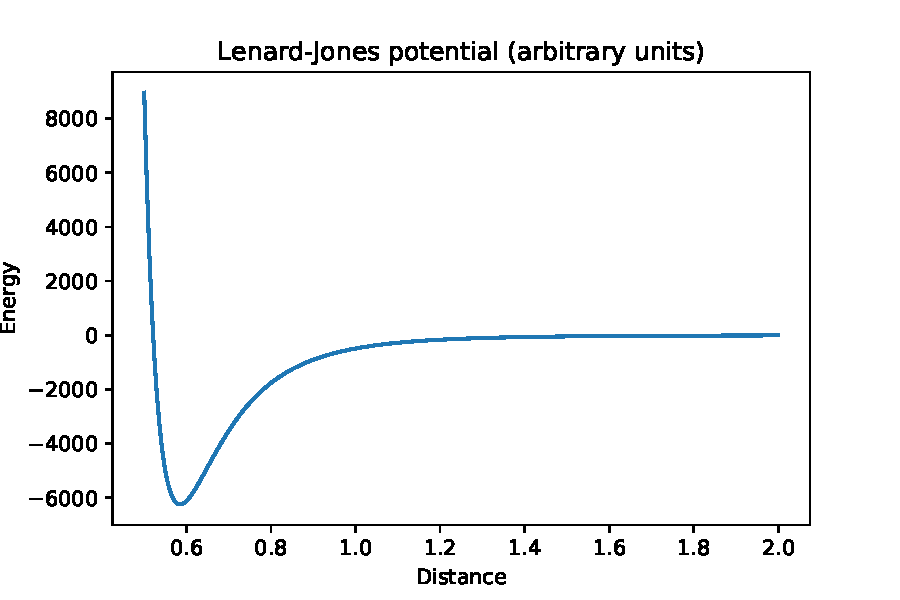
\includegraphics[clip,width=0.85\columnwidth]{LJ.pdf}%
}

\caption{Top: Schematic of atom-dimer collision, including all theinitial conditions variables. Bottom: Model of Lennard-Jones atom-atom pair potential.}
\label{fig:schematic}
\end{figure}


\subsection{\label{sec:level2}Numerical methods}

Talk about intergator used and maybe a quick tabel for convergence (change step size or delta t by a factor 2 and calculate some residual in the trajectory or check wehtehr the basin has changed).

\begin{figure}[htp]
\subfloat{
  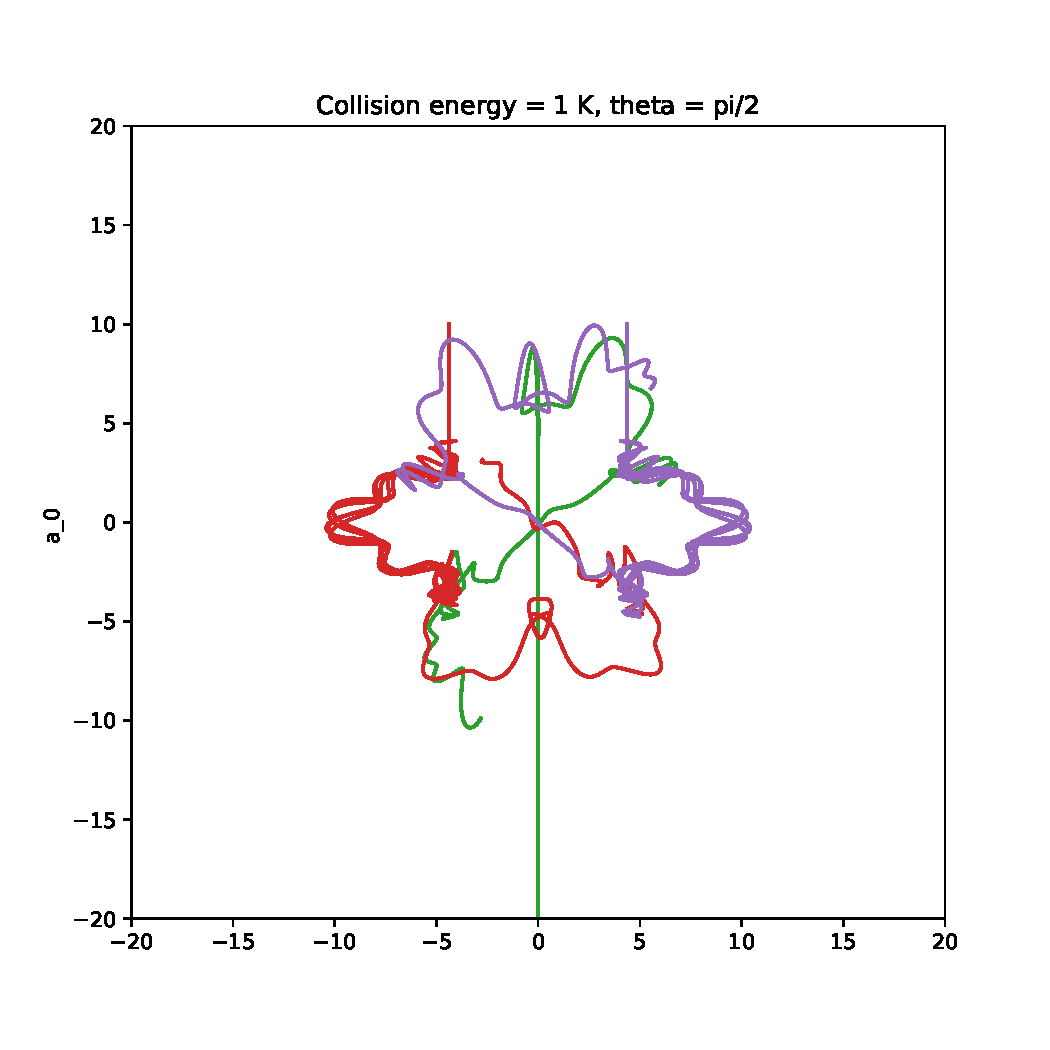
\includegraphics[clip,width=0.75\columnwidth]{traj_1.pdf}%
}

\subfloat{
  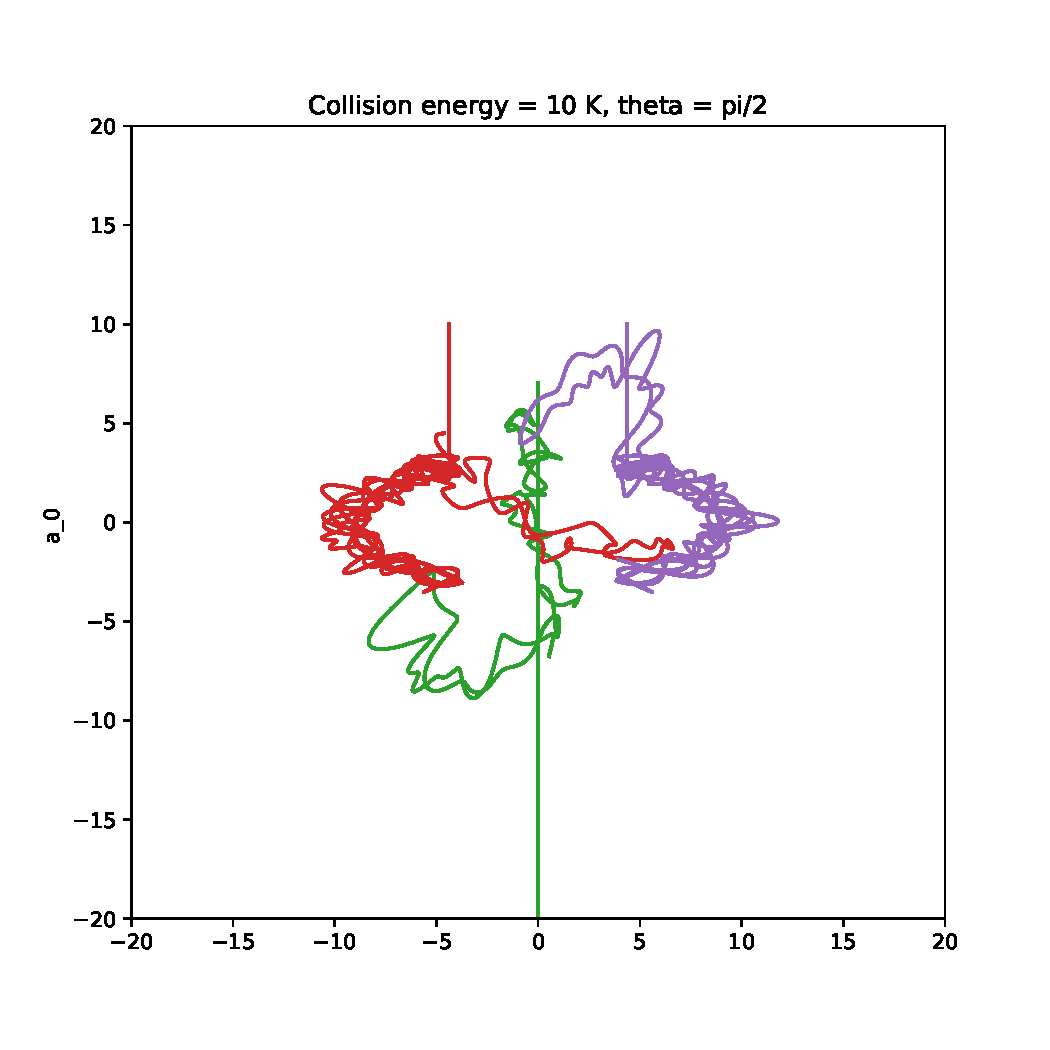
\includegraphics[clip,width=0.75\columnwidth]{traj_2.pdf}%
}

\subfloat{
  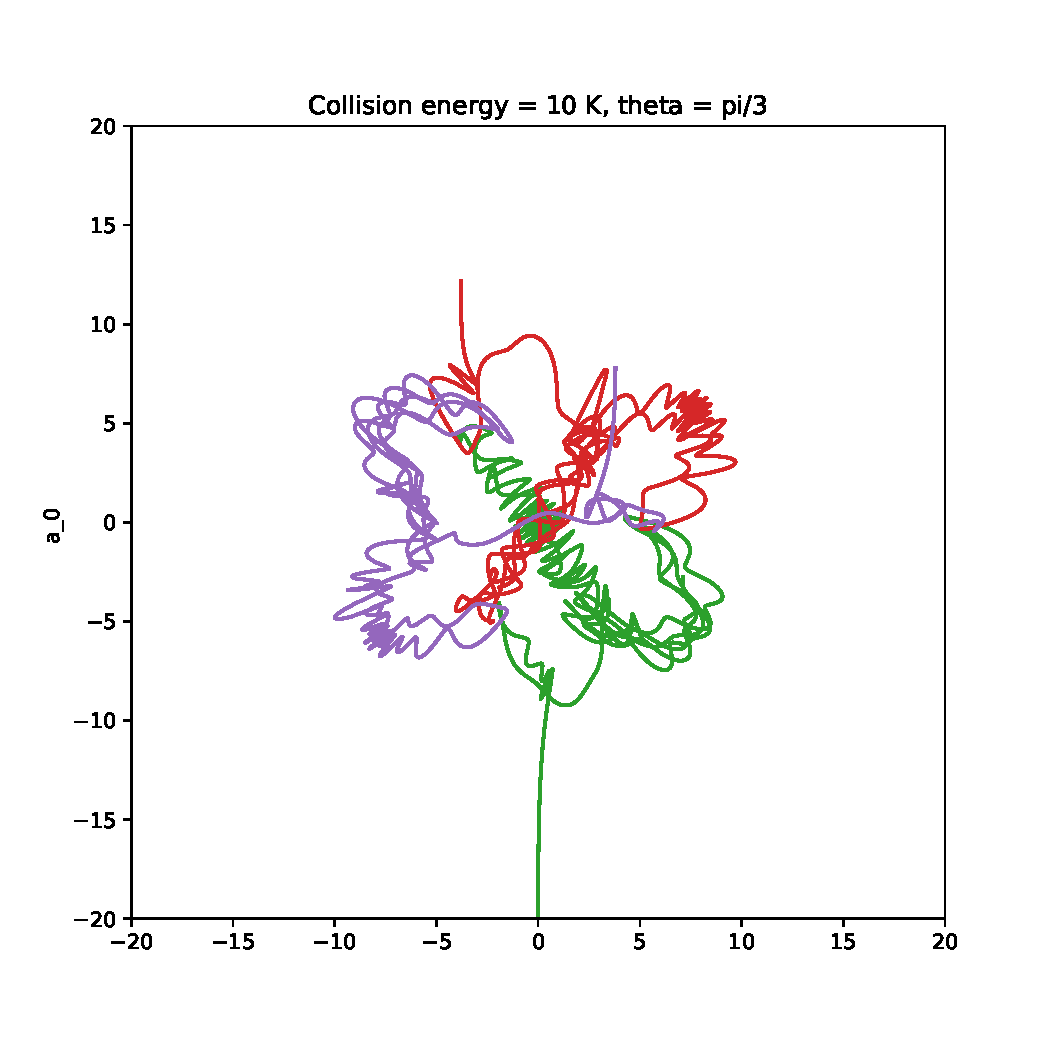
\includegraphics[clip,width=0.75\columnwidth]{traj_3.pdf}%
}

\caption{Top: Schematic of atom-dimer collision, including all theinitial conditions variables. Bottom: Model of Lennard-Jones atom-atom pair potential.}
\label{fig:schematic}
\end{figure}

\subsection{\label{sec:level2}Complex lifetime}

One of the main observables of interest in ultracold collisions is the complex' lifetime (or the related quantity of scattering rate), which can provide information about the ergodicity of the reaction and can also be cross-checked with other methods of analyzing the collision  {\color{red}Relate this to what Jessie did.I didn't quite get Fig. 2, which may be interesting and should be easy to get, if anyone else wants to do it. There is some code to do it. Otherwise, we should be fine; we don't have to replicate everything..}. To this end, we compute the lifetime of the reaction as the time between the initial starting point (the atom starts $r_{\mathrm{init}} = 60 a_0$ away from the dimer, where $a_{\mathrm{0}}$ is the Bohr radius and the equilibrium distance between the dimer's atoms is $\bar{a} = 8.78 a_{\mathrm{0}}$ and the time when the hyper-radius $\sqrt{R^2_{\mathrm{AB}} + R^2_{\mathrm{BC}} + R^2_{\mathrm{AC}}}$ is first greater than $ r_{\mathrm{init}}$. We note that different methods of timing the reaction are possible, but they should not change the functional behavior of the lifetime. In particular, we analyze the dependence of the lifetime as a function of the collision energy for two atom species, as shown in Fig.~\ref{fig:lifetime}. We observe that lifetime has a power-law dependence on the initial energy, with exponent $-0.47$ for $\mathrm{Li} + \mathrm{Li_{2}}$ and $-0.50$ for $\mathrm{Cs} + \mathrm{Cs_{2}}$.

\begin{figure}[ht]
\begin{center}
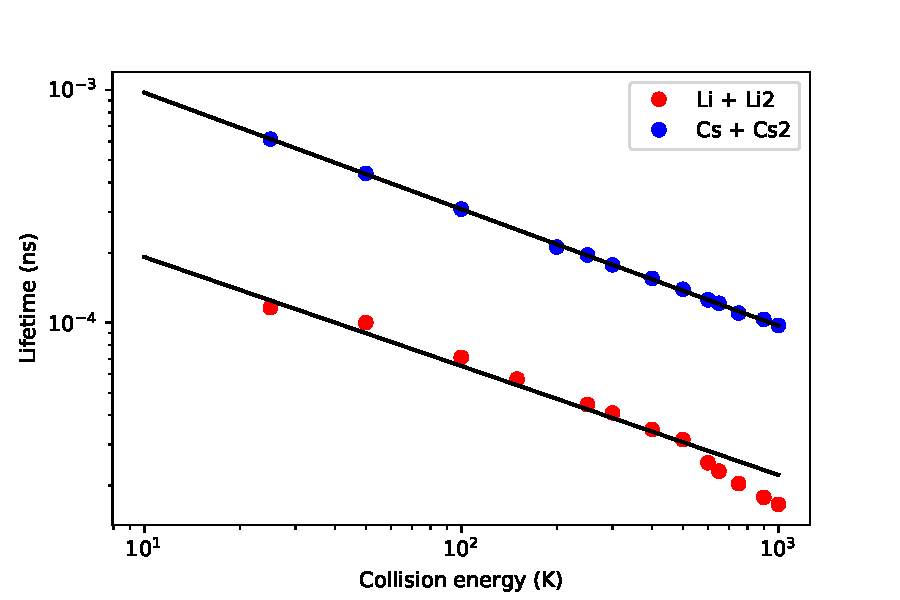
\includegraphics[width=1.1\linewidth]{lifetime.pdf}
\caption{Lifetime as a function of the collision energy for the atom-dimer cases of $Li + Li_2$ and $Cs + Cs_2$. The dots represent the computed total time that the atom-dimer pair spend in the reaction, while the solid line represents a power-law fit.}
\label{fig:lifetime}
\end{center}
\end{figure}

{\color{red}Maybe talk about ergodicity and applicability of RRKM but, again, I think this is more what Jessie did so maybe she will mention it. Otherwise can summariz page 4 from Bohn's paper here.}

\subsection{\label{sec:level3}Chaos}

An interesting feature of atomic-dimer dynamics at ultracold temperatures is the onset of chaos, which arises as the atoms get closer together in low-energy regimes and the interactions get stronger. We can observe the chaotic behvaior by analyzing the outcome of trajectories as a function of the initial conditions. We thus vary $\theta$, the angle of orientation of the dimer with respect to the velocity of the incoming atom, and look at both the lifetime of the trajectory as well at what "kind" of trajectories they are: similar to what Croft and Bohn did, we use the fact that this is a classical collision and can therefore label each atom involved; we thus classify trajectories by whether the two initial atoms forming the dimer stayed together (AB+C), whether they changed partners (AC+B or BC+A), or whether the complex broke apart with all three atoms flying apart independently (A+B+C).

The results for $\mathrm{Li} + \mathrm{Li_2}$ at $T = 350~\mathrm{K}$ are summarized in Fig.~\ref{fig:chaos}. We conclude that, while there are regions of relative stability, both the lifetime and the ending "basin" can vary wildly as a function of $\theta$. Even more compelling, by "zooming in" on a region of $\theta$ we qualitatively observe the same features, so we conclude that the system exhibits the scale invariance characteristic of fractals.

\begin{figure}[htp]
\subfloat{
  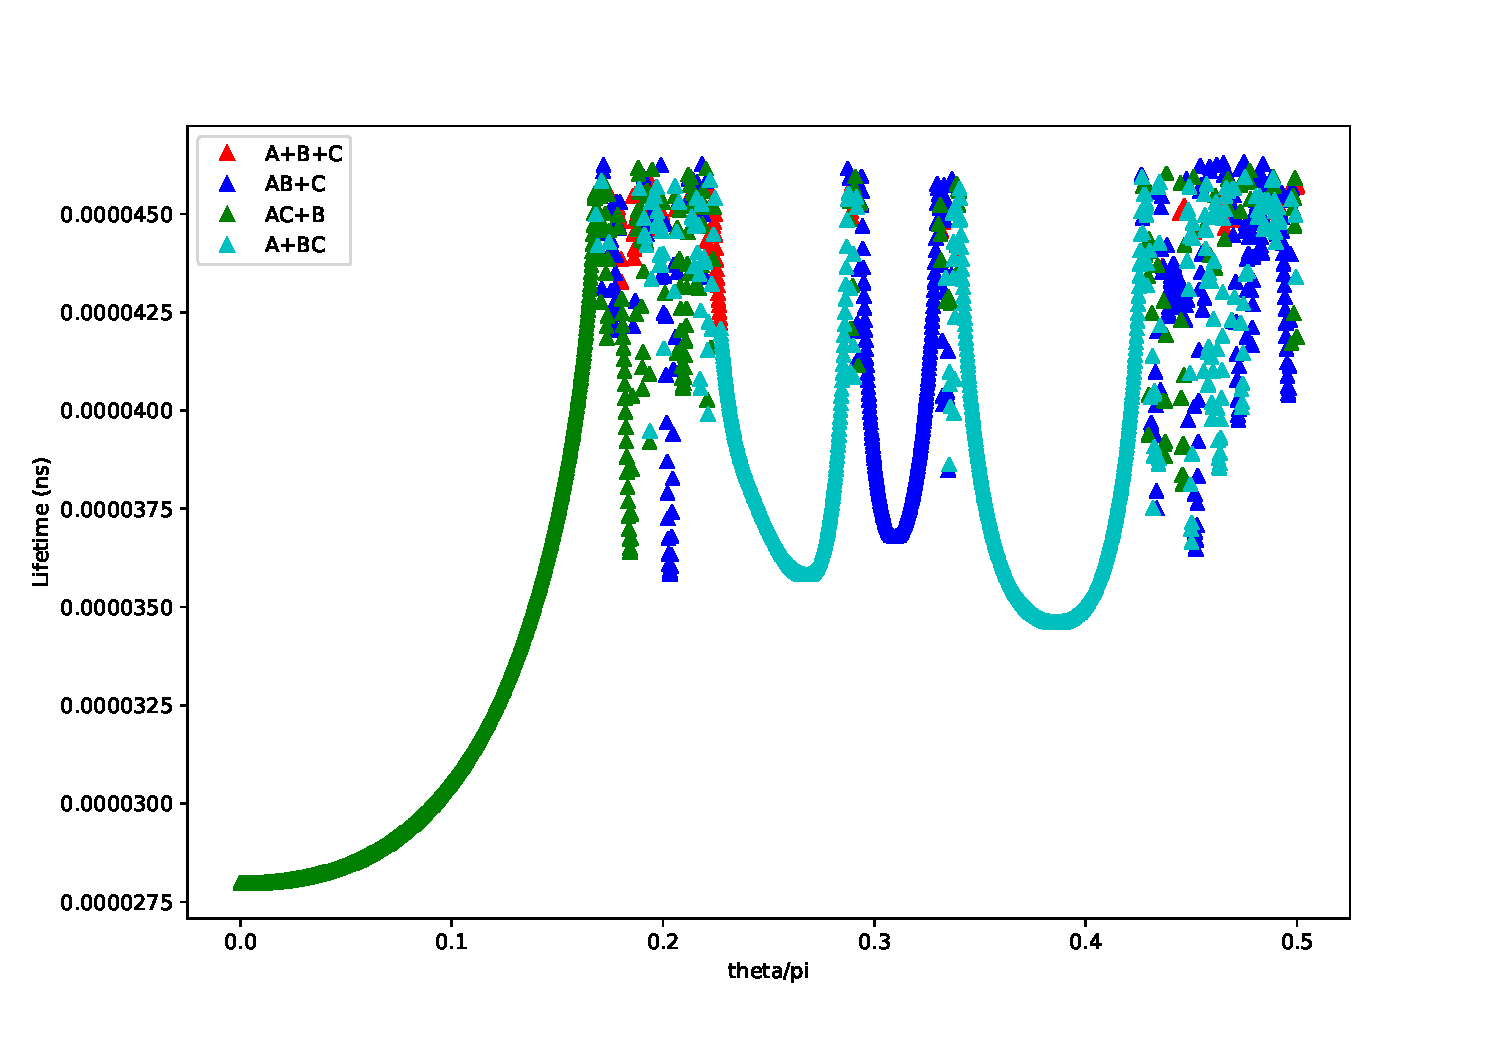
\includegraphics[clip,width=\columnwidth]{fractal_big.pdf}%
}

\subfloat{
  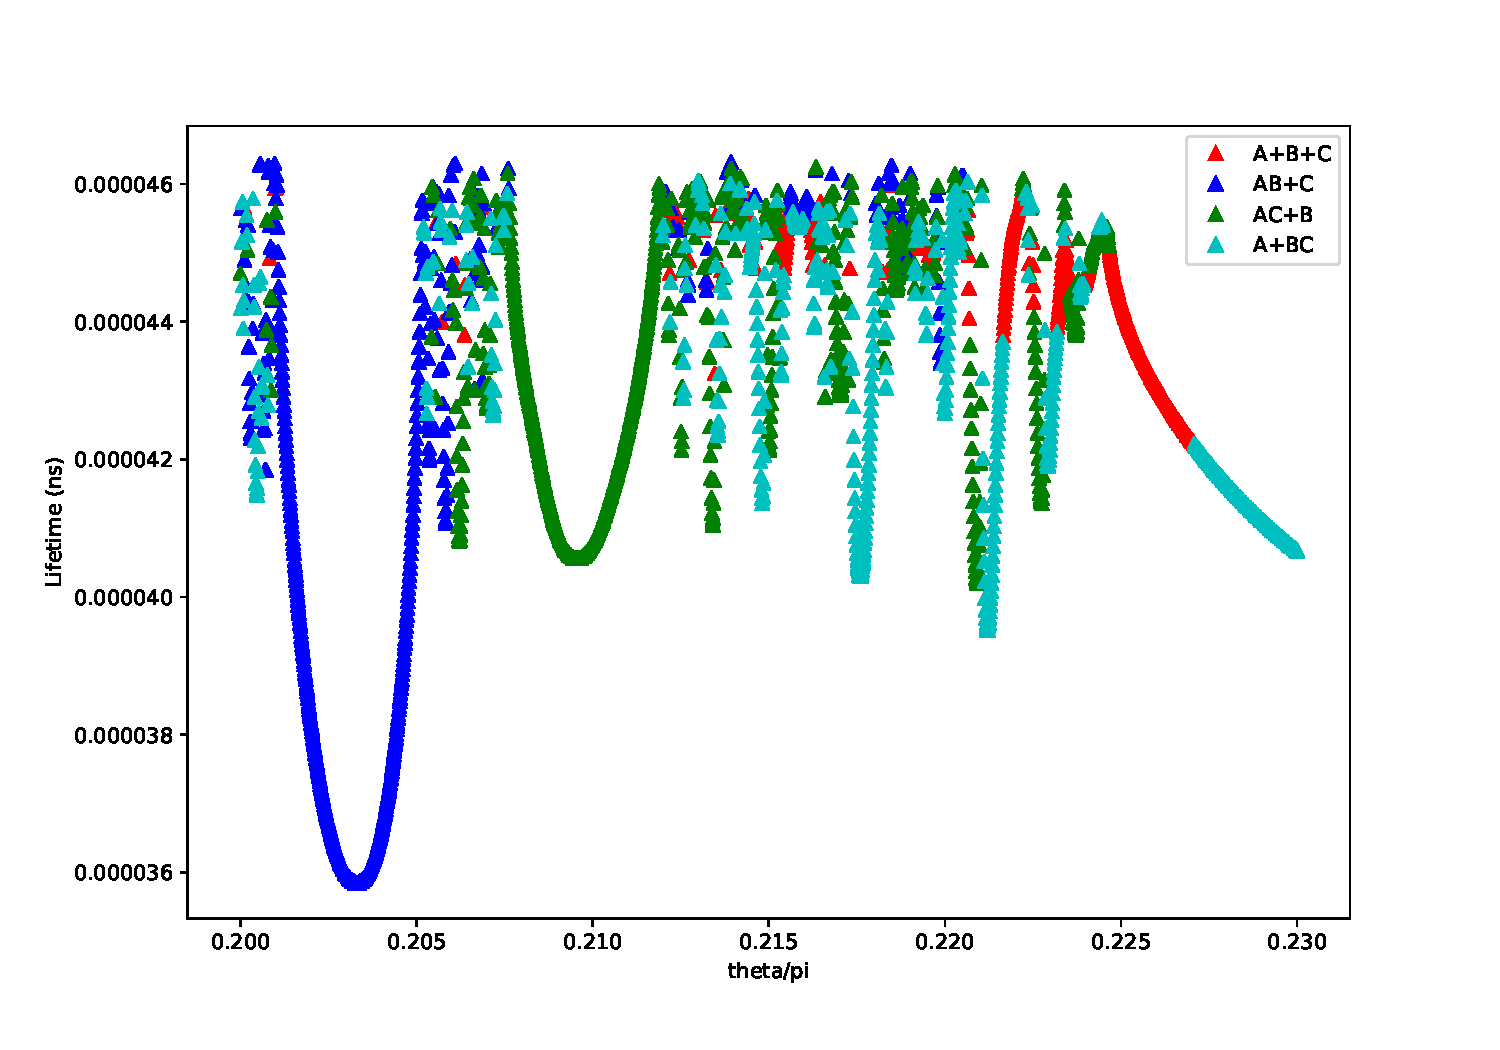
\includegraphics[clip,width=\columnwidth]{fractal_zoomed.pdf}%
}
\label{fig:chaos}
\caption{Lifetime and ending "basin"  for $\mathrm{Li} + \mathrm{Li_2}$ at $T = 350~\mathrm{K}$ as a function of the initial orietnation angle of the dimer $\theta$. The lower panel is a zoomed in version of the upper one, illustrating the scale invariance property of the system.
}
\end{figure}

The fractal dimension~\cite{mandelbrot1967} characterizes how much the fractal pattern changes as one changes the scale of the system, so it is a way to quantify the scale invariance and, as we shall see, also the moment of onset of chaos. As already discussed, we classify trajectories by the "basin" they end up in. A trajectory is further classified as unstable under perturbation of initial conditions if by changing the intial variables by a value $\delta$ the ourcome ends being part of a different basin than the original one. As such, we compute a large number of pair of trajectories, in each pair the partners having the initial conditons (in our case, the orietnation angle $\theta$) differ by an amount $\delta$. We then compute the fraction of unstable trajectories, which is observed to be characterized by the uncertainty algorithm~\cite{mcdonald1985}

\begin{equation}
f(\delta, E_{\mathrm{col}}) \propto \delta^{\alpha(E_{\mathrm{col}})},
\end{equation}
where $E_{\mathrm{col}}$ is the collision energy, $\delta$ is the perturbation we apply (to the angle $\theta$), and $\alpha$ is the uncertainty exponent that we fit.

Figure~\ref{fig:unc} illustrates some of the results for a wide range of temperatures, from which we can conclude that at high collision energies the trajectories are essentially stable under perturbation, with the unstable fraction decreasing as $\delta$ gets smaller, while for lower collision energies the unstable fraction is essentially independent of $\delta$, meaning that there is no correlation between the outcomes of trajectories that are arbitrarily closely "neighboring" in the phase space of initial conditions.

\begin{figure}[ht]
\begin{center}
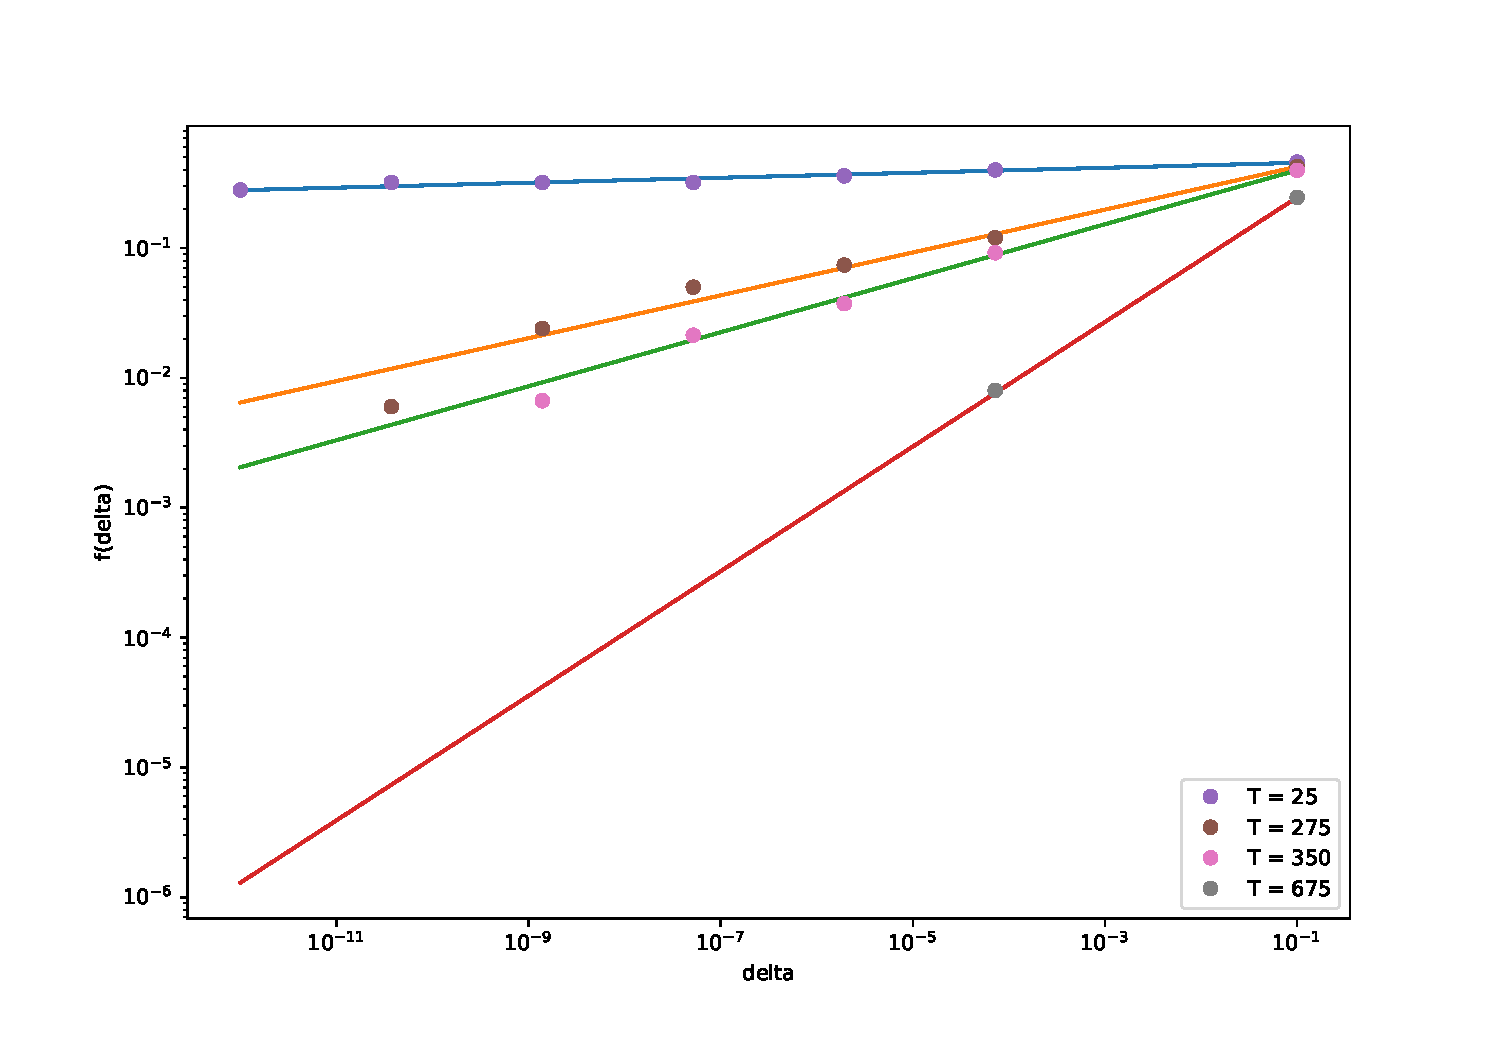
\includegraphics[width=1.05\linewidth]{uncertainty.pdf}
\caption{The unstable fraction of trajectories, $f(\delta)$, as a function of the perturbation value $\delta$ for $\mathrm{Li} + \mathrm{Li_2}$. At $25$ K $\alpha$ is $0.02$, corresponding to trajectories that are completely sensitive to initial conditions' perturbations, while at $250$ K and $675$ K it is $0.2$ and $0.48$, respectively.}
\label{fig:unc}
\end{center}
\end{figure}

Quickly talk about fractal dimension...

\begin{figure}[ht]
\begin{center}
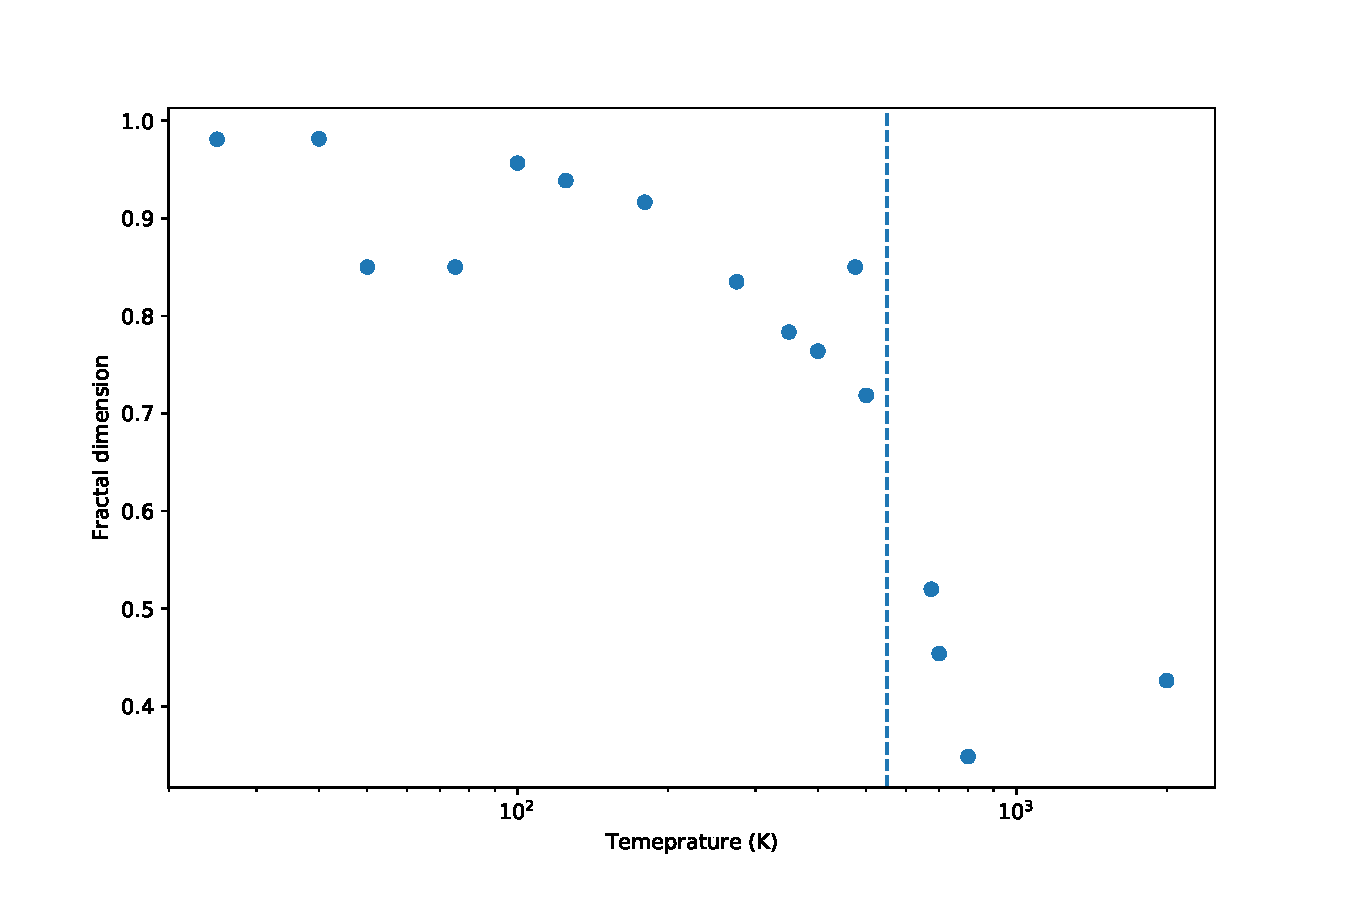
\includegraphics[width=1.05\linewidth]{fractal_dim.pdf}
\caption{Fractal dimension $d$ as a function of the collision energy of $\mathrm{Li} + \mathrm{Li_2}$. The vertical line marks the approximate energy at which chaotic behvior ensues.}
\label{fig:frac_dim}
\end{center}
\end{figure}

 
\begin{figure}[ht]
\begin{center}
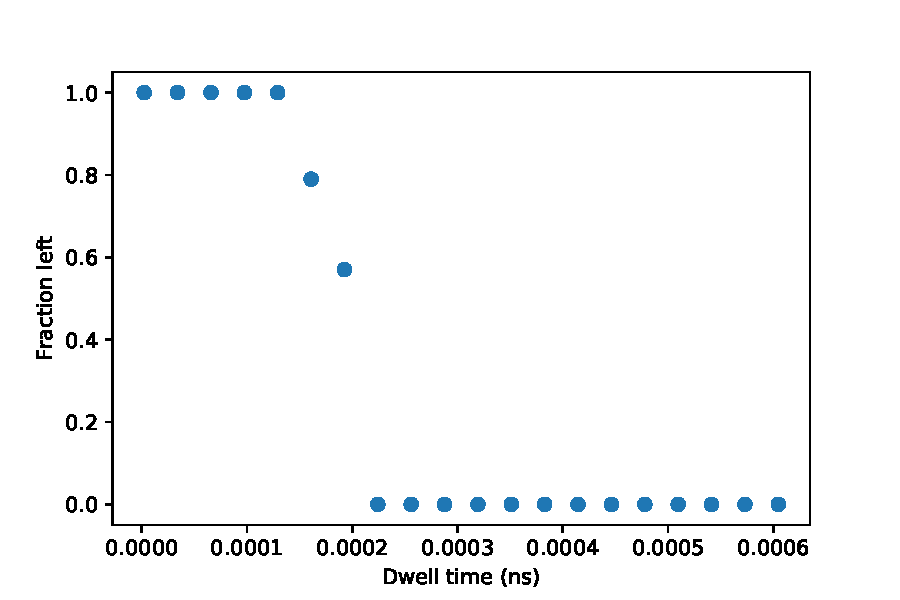
\includegraphics[width=1\linewidth]{fraction_left.pdf}
\caption{}
\label{fig:lifetime}
\end{center}
\end{figure}



%\begin{equation}
%  \frac{\p \rho}{\p t} = -\nabla \cdot \vec{j}
%\end{equation}
%and take the flux to be given by Fick's law, $\vec{j}=-\nabla\rho$, yielding
%the diffusion equation,
%\begin{equation}
%  \frac{\p \rho}{\p t} = \nabla^2 \rho. \label{eq:diff}
%\end{equation}
%Since time can be rescaled in the subsequent analysis, the diffusion constant
%in Fick's law is set to 1. Any tracers that are being carried by this density
%flux will move with velocity
%\begin{equation}
%  \vv(\vx,t) = \frac{\vec{j}}{\rho} = - \frac{\nabla \rho}{\rho}. \label{eq:vel}
%\end{equation}
%If Eq.~\ref{eq:diff} is solved to steady state, and the map is deformed
%according to the velocity field in Eq.~\ref{eq:vel}, then the final state of
%the map will have equalized density. To track the deformation of the map,
%Gastner and Newman introduce tracers $\vec{r}(t)$ that follow the velocity
%field according to
%\begin{equation}
%  \vec{r}(t) = \vec{r}(0) + \int_0^t \vv(\vec{r},t') dt'.
%\end{equation}
%
%\subsection*{The reference map technique for large-strain solid mechanics}
%Numerical methods for large-strain solid mechanics typically employ a
%Lagrangian computational perspective, where the solid is represented by a
%moving and deforming mesh, and the amount of mesh deformation can be used to
%construct the stress response of the solid. However, a fully Eulerian
%formulation would be advantageous in some situations, such as for
%fluid--structure interaction, since fluids usually make use of Eulerian
%approaches~\cite{tannehill97}.
%
%A fully Eulerian method for simulating large-strain solid mechanics has
%recently been developed~\cite{kamrin12,valkov15}. The key idea behind the
%method is to introduce a vector field $\bxi(\vx,t)$ called the
%\textit{reference map}, which is initialized at $t=0$ to be equal to the
%current spatial coordinate, so that $\bxi(\vx,0)=\vx$. The field is then
%advected according to a continuum velocity field $\vv(\vx,t)$ using the
%equation
%\begin{equation}
%  \frac{\p \bxi}{\p t} + (\vv \cdot \nabla) \bxi = \vec{0}. \label{eq:rmap}
%\end{equation}
%This field tracks how the solid has deformed: $\bxi(\vx,t)$ measures where the
%material that is currently at $(\vx,t)$ originated from. This field is very
%useful for large-strain solid mechanics since the deformation gradient tensor
%$\vec{F}$~\cite{lubliner08,gurtin10} is given by finite differences of $\bxi$, according
%to $\vec{F}=(\p \bxi/ \p \vx)^{-1}$. Coupling this to Newton's second law and a
%constitutive relation for the Cauchy stress, $\boldsymbol\sigma=f(\vec{F})$,
%gives a simple closed system of partial differential equations for $\bxi$ and
%$\vv$ that can be solved in an Eulerian finite-difference framework.
%
%\subsection*{An alternative map-making method}
%The reference map technique can be applied to the map-making problem, as an
%alternative approach to track how the map deforms. This involves coupling
%Eqs.~\ref{eq:diff} \& \ref{eq:vel} with Eq.~\ref{eq:rmap}. This was implemented
%in C++ using a simple, explicit formulation, using the domain $|x|\le 2, |y|
%\le 2$ where $\vx=(x,y)$. Two test problems on $200 \times 200$ grids were
%performed. The first uses an initial density of
%\begin{equation}
%  \rho(\vx,0) = \frac{1 + 9e^{-5|\vx|^2}}{10}
%\end{equation}
%and a sequence of simulation snapshots is shown in Fig.~\ref{fig:gauss}.
%The white lines in these snapshots are the contours of the components of the
%reference map and provide a simple method to visualize the deformation of the
%map. If a real map image of a country was being used, the deformed image could
%be constructed by coloring position $\vx$ using the color at $\bxi(\vx,t)$ in
%the original image.
%
%\setlength{\unitlength}{0.0125bp}
%\begin{figure}
%  \begin{center}
%    \small
%    \begin{picture}(33000,28600)(0,0)
%      \put(-1500,13500){\parbox{15cm}{\include{gauss_rho}}}
%      \setlength{\unitlength}{0.0125bp}
%      \put(30000,4700){ 
%	\begin{picture}(2000,21100)(0,0)
%	  \put(0,1600){\includegraphics[width=12.5pt,height=226pt]{colorchart_v}}
%	  \put(0,1600){\line(0,1){18000}}
%	  \put(0,1600){\line(1,0){1200}}
%	  \put(1000,1600){\line(0,1){18000}}
%	  \put(0,19600){\line(1,0){1200}}
%	  \put(500,400){\makebox(0,0)[c]{$\rho$}}
%	  \put(1000,6100){\line(1,0){200}}
%	  \put(1000,10600){\line(1,0){200}}
%	  \put(1000,15100){\line(1,0){200}}
%	  \put(1320,1600){\makebox(0,0)[l]{0}}
%	  \put(1320,6100){\makebox(0,0)[l]{\nicefrac{3}{10}}}
%	  \put(1320,10600){\makebox(0,0)[l]{\nicefrac{6}{10}}}
%	  \put(1320,15100){\makebox(0,0)[l]{\nicefrac{9}{10}}}
%	  \put(1320,19600){\makebox(0,0)[l]{\nicefrac{12}{10}}}
%	\end{picture}}
%    \end{picture}
%  \end{center}
%  \vspace{6mm}
%  \caption{Four snapshots of the density field $\rho(\vx,t)$ in a
%  density-equalizing reference map calculation starting from a gaussian initial
%  condition. The thin white lines are the contours of the components of
%  the reference map $\bxi(\vx,t)$ and show how the map has deformed to equalize
%  the density.\label{fig:gauss}}
%\end{figure}
%
%The second test problem considered uses the initial density
%\begin{equation}
%  \rho(\vx,0)=\left\{
%  \begin{array}{ll}
%    \nicefrac{1}{4} & \qquad \text{if $x<0$ and $y<0$,} \\
%    1 & \qquad \text{if $x<0$ and $y\ge 0$,} \\
%    \nicefrac{3}{4} & \qquad \text{if $x\ge0$ and $y<0$,} \\
%    \nicefrac{1}{2} & \qquad \text{if $x\ge0$ and $y\ge0$.}
%  \end{array}
%  \right.
%\end{equation}
%A sequence of simulation snapshots is shown in
%Fig.~\ref{fig:checker}.
%
%\setlength{\unitlength}{0.0125bp}
%\begin{figure}
%  \begin{center}
%    \small
%    \begin{picture}(33000,28600)(0,0)
%      \put(-1500,13500){\parbox{15cm}{\include{checker_rho}}}
%      \setlength{\unitlength}{0.0125bp}
%      \put(30000,4700){ 
%	\begin{picture}(2000,21100)(0,0)
%	  \put(0,1600){\includegraphics[width=12.5pt,height=226pt]{colorchart_v}}
%	  \put(0,1600){\line(0,1){18000}}
%	  \put(0,1600){\line(1,0){1200}}
%	  \put(1000,1600){\line(0,1){18000}}
%	  \put(0,19600){\line(1,0){1200}}
%	  \put(500,400){\makebox(0,0)[c]{$\rho$}}
%	  \put(1000,6100){\line(1,0){200}}
%	  \put(1000,10600){\line(1,0){200}}
%	  \put(1000,15100){\line(1,0){200}}
%	  \put(1320,1600){\makebox(0,0)[l]{0}}
%	  \put(1320,6100){\makebox(0,0)[l]{\nicefrac{3}{10}}}
%	  \put(1320,10600){\makebox(0,0)[l]{\nicefrac{6}{10}}}
%	  \put(1320,15100){\makebox(0,0)[l]{\nicefrac{9}{10}}}
%	  \put(1320,19600){\makebox(0,0)[l]{\nicefrac{12}{10}}}
%	\end{picture}}
%    \end{picture}
%  \end{center}
%  \vspace{6mm}
%  \caption{Four snapshots of the density field $\rho(\vx,t)$ in a
%  density-equalizing reference map calculation starting from a $2\times 2$
%  checkered initial condition. The thin 
%  white lines are the contours of the components of the reference map
%  $\bxi(\vx,t)$ and show how the map has deformed to equalize the
%  density.\label{fig:checker}}
%\end{figure}
%
%\subsection*{A possible simplification}
%Mathematically, the density field at time $t$ is given in terms of the
%reference map according to
%\begin{equation}
%  \rho(\vx,t) = \rho(\bxi(\vx,t),0) \det \left( \frac{\p \bxi}{\p \vx}\right). 
%\end{equation}
%It may therefore be possible to formulate a numerical scheme dependent solely
%on $\bxi(\vx,t)$, without the need to track $\rho$ as a separate field.

\bibliography{elect}
\end{document}
